\section{Neural Networks and Deep Learning}

%%%%%%%%%%%%%%%%%%%%%%%%%%%
%%%%%%%%%%%%%%%%%%%%%%%%%%%
%%%%%%%%%%%%%%%%%%%%%%%%%%%
%%%%%%%%%%%%%%%%%%%%%%%%%%%
%%%%%%%%%%%%%%%%%%%%%%%%%%%
\subsection{Introduction}

A neural network is a ML model inspired by the network of biological neurons in our brains.

NNs are versatile, powerful, and scalable.
Consequently, they frequently outperform other ML techniques on very large and complex problems.
NNs are at the very core of Deep Learning.

\textbf{Threshold Logic Units (TLUs)} are the building block of neural networks (i.e. the neurons):
\begin{itemize}
\vspace{-4.0mm}

\item
First, they perform a weighted sum of the inputs, $z = \sum w_i x_i$

\item
\vspace{-2.0mm}
Then they apply an \textit{activation function} to that sum, $h_{\boldsymbol{w}}(\boldsymbol{x}) = \phi(z)$, and output the result.\newline
\begin{figure}[ht]
\centering
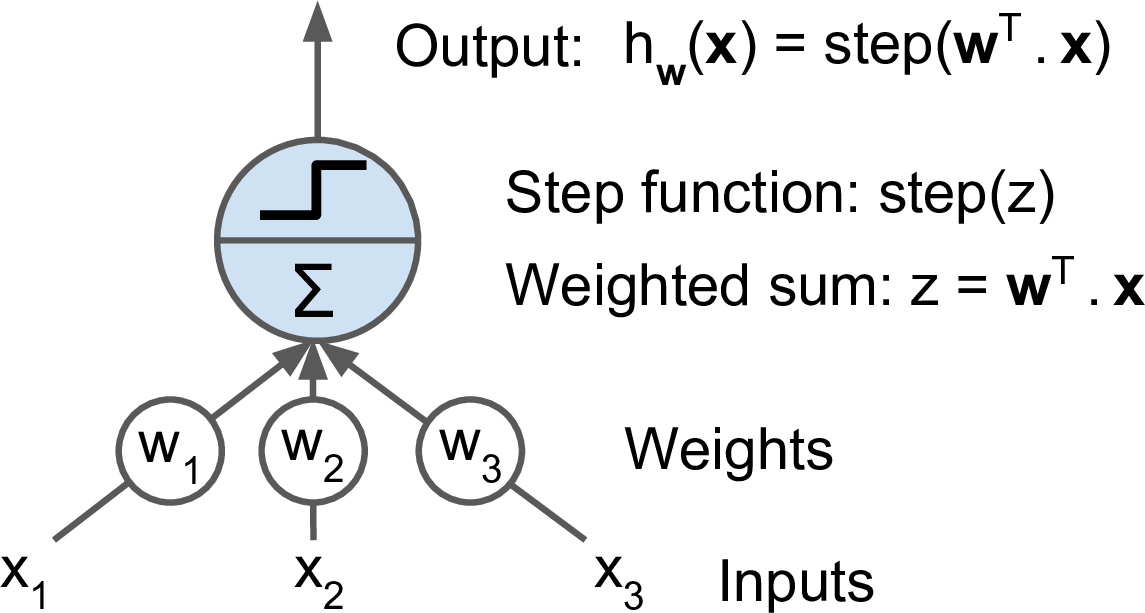
\includegraphics[width=0.50\textwidth]{./images/TLU.png}
\end{figure}

\item
\vspace{-2.0mm}
Traditionally, the activation function was a heavyside step function.
However, in order to perform Gradient Descent on a NN,
a differentiable function was needed instead.\newline
- The default has become the Rectified Linear Unit functoin: ReLU(z) = max(0,z)\newline
- The logistic function and hyperbolic tangent function are also popular choices.
\end{itemize}
\vspace{-2.0mm}


\textbf{Multilayer Perceptrons (MLPs)} are composed of multiple TLUs as depicted in the diagram.\newline
\textit{The bias neurons are shown, but usually they are implicit.}
\begin{figure}[ht]
\centering
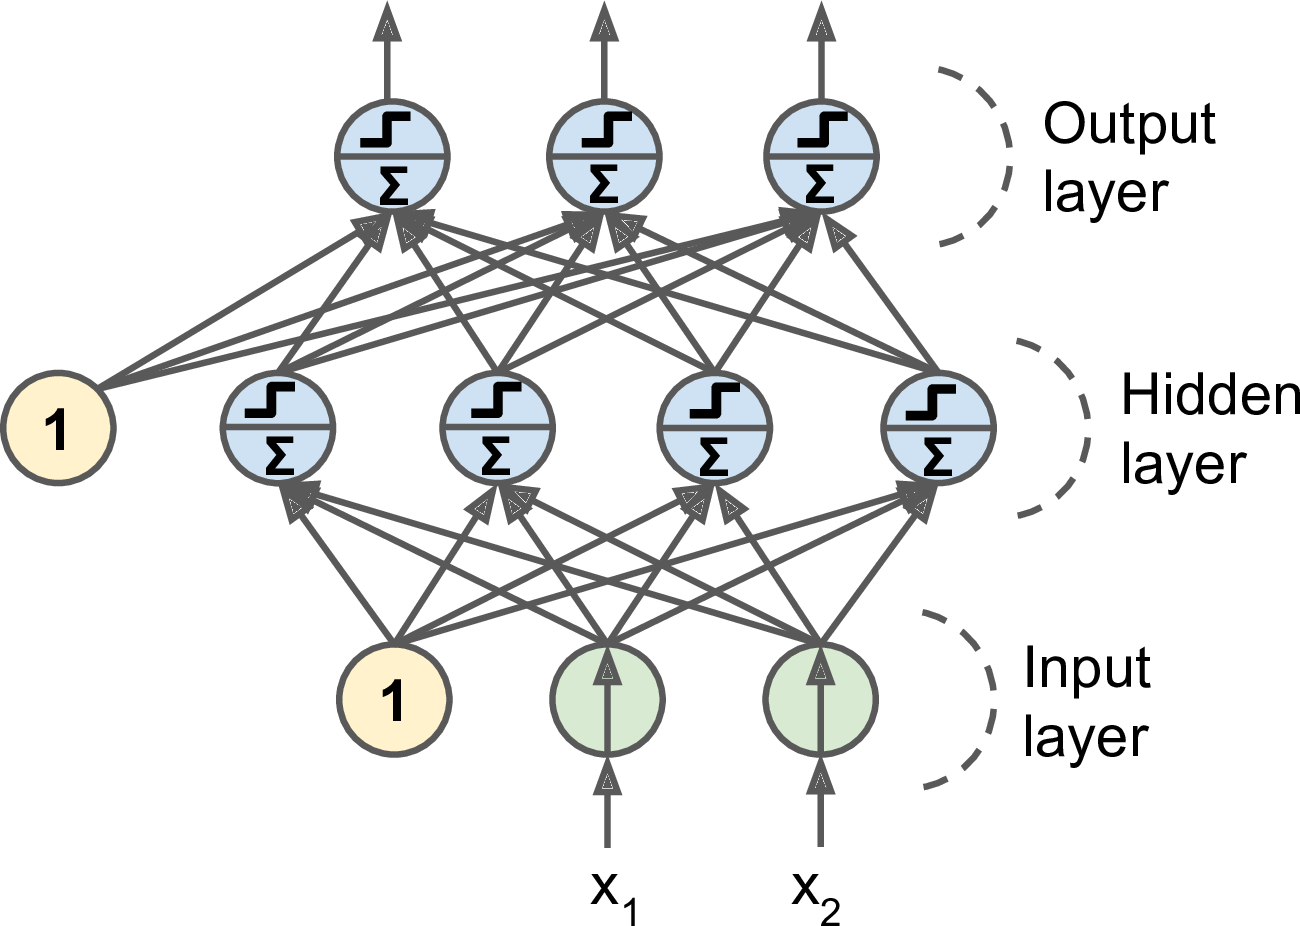
\includegraphics[width=0.50\textwidth]{./images/MLP.png}
\end{figure}

\vspace{-6.0mm}
\begin{itemize}
\item
When there's a deep stack of hidden layers, it is called a \textit{deep neural network (DNN)}.
\item
\vspace{-2.0mm}
Layers close to the input layer are called the \textit{lower layers}\newline
Layers close to the output layer are called the \textit{upper layers}.
\item
\vspace{-2.0mm}
When all the neurons in a layer are connected to every neuron in the previous layer,\newline
the layer is called a \textit{fully connected layer} or a \textit{dense layer}.
\item
\vspace{-2.0mm}
The signal flows only in one direction $=$ \textit{feedforward neural network (FNN)}.
\item
\vspace{-2.0mm}
Without the activation functions, all you would get is a linear model!
\end{itemize}

\newpage
\textbf{Training NNs: Backpropagation}.\newline
In just two passes through the network (one forward, one backward)
the backpropagation algorithm is able to compute the gradient of the network's error
with regard to every single model parameter (i.e. the connection weights),
allowing Gradient Descent to be used to train the NN.

\vspace{-5.0mm}
\begin{itemize}
\item
It handles one mini-batch at a time. The bigger the batch size, the more memory required.

\item
\vspace{-2.0mm}
\textit{The forward pass}.
Each mini-batch is passed through the network.
The output of every neuron is computed and preserved (for every instance in the mini-batch).

\item
\vspace{-2.0mm}
The network's output error is measured.

\item
\vspace{-2.0mm}
\textit{The reverse pass}.
The error gradient across all the connection weights is measured
by propagating the error gradient backward through the network.

\item
\vspace{-2.0mm}
an \textbf{iteration} = one forward-backward pass using one mini-batch.\newline
an \textbf{epoch} = one forward-backward pass of \textit{all} the training set examples.\newline
If you have 2000 training examples, and your batch size is 500\newline
$\rightarrow$ then it will take 4 iterations to complete 1 epoch.

\item
\vspace{-2.0mm}
It is important to randomly initialize all the hidden layer's connection weights.\newline
This breaks the symmetry and allows backpropagation to train a diverse team of neurons.

\end{itemize}

\textbf{Regression MLPs: Summary}

\begin{tabular}{ |l|l| } 
\hline
Hyperparameter & Typical value \\ 
\hline
Number of input neurons & One per input feature \\ 
Number of hidden layers & Depends on the problem, but typically 1 to 5\\ 
Number of neurons per hidden layer & Depends on the problem, but typically 10 to 100\\ 
Hidden layer activation function & ReLU or SELU\\
Number of output neurons & 1 per prediction dimension\\
Output activation function & In general None (can output any range of values)\\
 & ReLU/softplus (for a positive output contraint)\\
 & Logistic/tanh (for a bounded output contraint)\\
Loss function & Typically MSE (mean squared error)\\
 & Maybe MAE (mean absolute error) when there's lots of outliers\\
\hline
\end{tabular}

\textbf{Classification MLPs: Summary}

\begin{tabular}{ |l|l| } 
\hline
Hyperparameter & Typical value \\ 
\hline
Number of input neurons & One per input feature \\ 
Number of hidden layers & Depends on the problem, but typically 1 to 5\\ 
Number of neurons per hidden layer & Depends on the problem, but typically 10 to 100\\ 
Hidden layer activation function & ReLU or SELU\\
Number of output neurons & 1 (for binary classification)\\
 & 1 per class (for multiclass classification)\\
Output activation function & Logistic (for binary classification)\\
 & Softmax (for multiclass classification)\\
Loss function & Cross entropy\\
\hline
\end{tabular}

\newpage
The architecture of an MLP for multiclass classification:

\begin{figure}[ht]
\centering
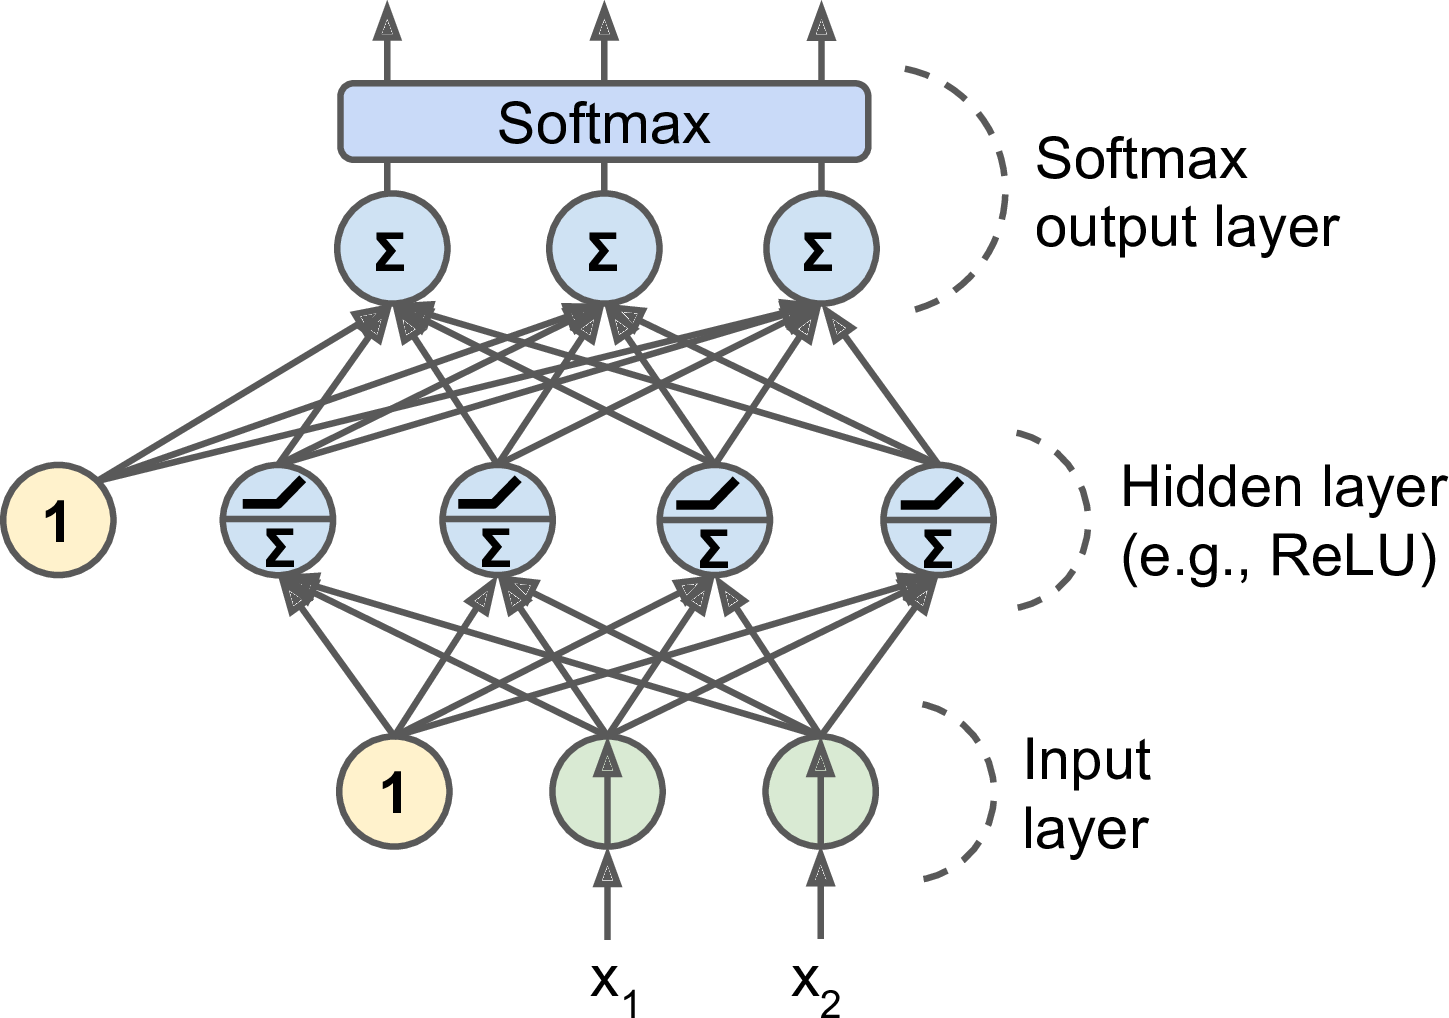
\includegraphics[width=0.50\textwidth]{./images/MLP_classification.png}
\end{figure}

%%%%%%%%%%%%%%%%%%%%%%%%%%%
%%%%%%%%%%%%%%%%%%%%%%%%%%%
%%%%%%%%%%%%%%%%%%%%%%%%%%%
%%%%%%%%%%%%%%%%%%%%%%%%%%%
%%%%%%%%%%%%%%%%%%%%%%%%%%%

up to page 295

\subsection{Keras Intro}

TODO
TODO
TODO
TODO
TODO
TODO
TODO
TODO

TODO
TODO
TODO
TODO
TODO
TODO
TODO
TODO

TODO
TODO
TODO
TODO
TODO
TODO
TODO
